
\section{Algorithms} \label{sec:algorithms}

As a means of producing fewer energy violations when scheduling system tasks, we have developed two techniques for reducing energy violations when scheduling tasks.  They are called the \emph{Smooth to Average Method} (\textsc{STAM}) and \emph{Smooth to Full Utilization} (\textsc{STFU}). 
\begin{figure}[htb]
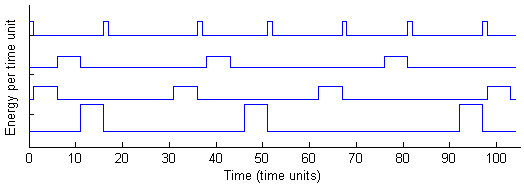
\includegraphics[scale=0.72]{edftasks.png}
\label{fig:edftasksched}
\caption{Four tasks scheduled by EDF with no smoothing.}
\end{figure}
\subsection{Smooth to Average Method}
The STAM heuristic takes into account the average energy requirements per unit time of all tasks in a given task list. We generate a set of equivalent \emph{virtual tasks} by increasing the duration of any task that uses greater than average energy per unit time, thus \emph{smoothing} each task to approximately the average energy per time unit. In these virtual tasks, the total energy remains the same as that in the real tasks, but it is spread over a longer duration.  

When the virtual task list has been created by STAM, the virtual tasks are scheduled by a known scheduling algorithm.  Virtual tasks cannot be scheduled to run at the same time and are not preemptible.  Once the virtual tasks are scheduled, the real tasks are inserted at the end of the corresponding virtual task's timeslot.  Thus a real task that consumes high energy is guaranteed to run after an idle period, which reduces the likelihood that the system will run out of energy when the task runs.

\begin{algorithm}[htb]
\label{stamalg}
\begin{algorithmic}
\STATE INPUT: $realTasks$ \COMMENT {list of [period, duration, energy]} 
\STATE INPUT: $N$ \COMMENT {number of tasks}
\STATE OUTPUT: $vTasks$ \COMMENT {same format as $realTasks$}
\STATE $E_{mean} \gets mean(realTasks[:,3])$
\FOR{$i = 1$ \TO $N$}
\IF{$taskList[i,3] > E_{mean}$}
\STATE $E_i \gets realTasks[i, 2] \times realTasks[i,3]$
\STATE $D_V \gets \lceil \frac{E_i}{E_{mean}} \rceil$
\STATE $E_V \gets \frac{E_i}{D_V}$
\STATE $vTasks[i,:] \gets [taskList[i,1]~~D_V~~E_V]$
\ELSE
\STATE $vTasks[i,:] \gets taskList[i,:]$
\ENDIF
\ENDFOR
\end{algorithmic}
\caption{Generate \textsc{STAM} Task List}
\end{algorithm}

The \textsc{STAM} algorithm calculates the energy consumption of each task by multiplying its runtime by the task's energy consumption per time unit. After taking the mean energy consumption across all of the tasks in the task list, each task is compared to the this value and virtual tasks are generated accordingly. If the given task's energy consumption is above the mean energy value, the virtual duration is calculated by taking the ceiling of the energy area of the task divided by the calculated energy mean. This will extend the duration of the virtual task allowing the total energy consumed to be more evenly distributed across the duration of the task's runtime. If the given task's energy consumption is below the calculated energy mean, the algorithm is unable to perform any smoothing and  will use the unchanged physical task to generate a schedule.
\begin{figure}[htb]
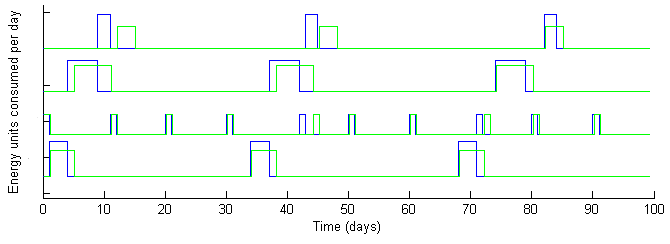
\includegraphics[scale=0.72]{stamtasks.png}
\caption{Four tasks scheduled by EDF with STAM smoothing}
\label{fig:stamtaskplot}
\end{figure}

\subsection{Smooth to Full Utilization}
The \textsc{STFU} algorithm is similar to STAM, but instead of smoothing all tasks to the average energy usage \textsc{STFU} attempts to create a virtual task list with 100\% \emph{virtual utilization}, $U_V$.  In other words, in a schedule generated from a virtual task list output by \textsc{STFU}, the likelihood of there being a virtual task scheduled at any arbitrary time is as close as possible to 100\%.

Utilization $U$ is defined in equation~\ref{eqn:utilization}, where $k$ is the number of tasks, $D_i$ is the duration of the $i^{th}$ task, and $P_i$ is the period of the $i^{th}$ task.
\begin{equation}
\label{eqn:utilization}
U = \sum_{i=1}^{k} \frac{D_i}{P_i}
\end{equation}
As $U \to 100\%$, EDF becomes the optimal scheduling algorithm regardless of energy. [nrqm - is this correct?]

To generate a virtual task list with \textsc{STFU}, first each task is given a virtual duty cycle $d_V$ representing what proportion of the total run time will be allocated to the corresponding virtual task.  The goal of \textsc{STFU} is to allocate more time to tasks that use greater energy, so that the system has more time to harvest energy before executing a high-energy task.  For example, a task that uses $40\%$ of the total energy consumed by tasks should be given a virtual duty cycle of $d_V=40\%$.  Virtual tasks cannot have a shorter duration than their real equivalents (otherwise the real task would not fit in the virtual task's timeslice), so if a task's real duty cycle $d$ is greater than $d_V$ then it will be unchanged.

This may lead to overutilization in rare cases.  In our simulation we ignore this issue; task lists are generated statically, so a system should not be programmed with a task list that is unschedulable.  When our tests encounter a randomly-generated task list that has $U > 100\%$ or $U_V > 100\%$), it generates new task lists until it gets one that is schedulable.
\begin{algorithm}[htb]
\label{alg:stfualg}
\begin{algorithmic}
\STATE INPUT: $realTasks$ \COMMENT {list of [period, duration, energy]} 
\STATE INPUT: $N$ \COMMENT {number of tasks}
\STATE OUTPUT: $vTasks$ \COMMENT {same format as $realTasks$}
\STATE $E_{total} = 0$
\FOR{$i = 1$ \TO $N$}
\STATE $d_i \gets \frac{realTasks[i, 2]}{realtasks[i,1]}$
\STATE $E_i \gets d_i \times realTasks[i,3]$
\STATE $E_{total} \gets E_{total} + E_i$
\ENDFOR
\FOR{$i = 1$ \TO $N$}
\STATE $d \gets \frac{E_i}{E_{total}}$
\STATE $d_{V} \gets max(realTasks[i, 2], \left \lfloor realtasks[i, 1] \times d \right \rfloor)$
\STATE $E_V \gets \frac{realTasks[i,2]\times realTasks[i,3]}{d_{V}}$
\STATE $vTasks[i] \gets [realTasks[i,1]~~d_{V}~~E_V]$
\ENDFOR
\end{algorithmic}
\caption{Generate \textsc{STFU} Task List}
\end{algorithm}

Figure~\ref{fig:stfutaskplot} shows four tasks scheduled by EDF with \textsc{STFU} smoothing.  Like in STAM, each real task is scheduled at the end of its virtual equivalent's time slice.  The third task, which uses the most energy over a long run, is scheduled after a long period spent collecting energy.  The second task uses very little energy overall, and is given just a short period to collect energy.  For the task set shown, $U \approx 27\%$ and $U_V \approx 96\%$.

\begin{figure}[htb]
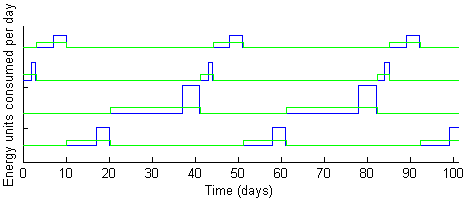
\includegraphics[scale=0.72]{stfutasks.png}
\caption{Four tasks scheduled by EDF with \textsc{STFU} smoothing}
\label{fig:stfutaskplot}
\end{figure}



































